% !TeX spellcheck = es_ES
% !TEX encoding = UTF-8 Unicode
\documentclass[t, compress, spanish, aspectratio=169]{beamer}
%\documentclass[handout]{beamer}    % for the handout

\usetheme[progressbar=frametitle]{metropolis}

\setbeamertemplate{navigation symbols}{} % Gets rid of navigation symbols

\usepackage{dsfont} % Double stroke fonts for math symbols
\usepackage[english]{babel} % Manages differences between languages: hyphenation etc
\addto\captionsenglish{\renewcommand{\figurename}{Figura}\renewcommand{\tablename}{Tabla}} % Spanish caption labels

\usepackage{appendixnumberbeamer} % Does not include backup slides in the number of pages

\usepackage{centernot} % To draw not in math symbols (does not imply)

\usepackage{ragged2e}  % Text alignment
\justifying

\usepackage{graphicx} % Format for graphics: additional options for includefigure
\usepackage{pgf} % Tool for graphics

\usepackage{booktabs} % Format for tables: top, bottom and mid lines
\usepackage[scale=2]{ccicons}
\usepackage{threeparttable} % Format for tables
\usepackage{lscape} % Landscape for tables

% Customized commands
  \newcommand{\vs}{\vskip0pt plus.5fill}
  \newcommand{\SR}{\mathbb{R}}
  \DeclareMathOperator{\plim}{plim}
  \DeclareMathOperator{\Var}{Var}
  \DeclareMathOperator{\Avar}{AVar}
  \DeclareMathOperator{\Cov}{Cov}
  \DeclareMathOperator{\N}{Normal}
  \DeclareMathOperator{\E}{\mathbb{E}}
  \DeclareMathOperator{\LP}{\mathbb{L}}
  \newcommand{\pto}{\stackrel{p}{\longrightarrow}}
  \newcommand{\dto}{\stackrel{d}{\longrightarrow}}
  \newcommand{\adistr}{\stackrel{a}{\sim}}
  \newcommand{\epsi}{\varepsilon}
  \newcommand\independent{\protect\mathpalette{\protect\independenT}{\perp}}
  \def\independenT#1#2{\mathrel{\rlap{$#1#2$}\mkern2mu{#1#2}}}
  \newcommand{\term}[1]{\structure{\textbf{#1}}} % label/definition markup, distinct from \alert (reserved for genuine callouts)


\title [Servicio militar e ingresos] {An\'alisis Econom\'etrico\\
	Servicio militar e ingresos:\\ regresi\'on simple, m\'ultiple y sesgo de variable omitida}
\author[de Elejalde]{Ramiro de Elejalde}
\institute [UAH] {Facultad de Econom\'ia y Finanzas \\ Universidad Alberto Hurtado}
\date[\today] {}
\subject{An\'alisis Econom\'etrico}
\begin{document}

	%------------------------------------------------------------

	\begin{frame}
		\titlepage
	\end{frame}

	% --------------------------------------------------- Slide --
	\begin{frame}
		\frametitle{Outline}
		\footnotesize
		\tableofcontents
		\alert{Referencias}: Angrist (1998, Econometrica); cap. 3.3.1 de Angrist y Pischke; clase 4 (Estimaci\'on por MCO), secci\'on de sesgo de variable omitida.
	\end{frame}

	% ============================================================
	\section{La pregunta y los datos}
	% ============================================================

	% --------------------------------------------------- Slide --
	\begin{frame}
		\frametitle{?`Sirve el servicio militar para ganar m\'as?}
		\begin{itemize}
			\item \term{Pregunta}: ?`Cu\'al es el efecto de servir en las fuerzas armadas sobre los ingresos posteriores de un solicitante?
			\item Es una pregunta de pol\'itica: el reclutamiento voluntario cuesta recursos p\'ublicos y los solicitantes deciden si ingresan o no.
			\item Comparar los ingresos de veteranos y no veteranos es lo obvio. \alert{Pero la comparaci\'on mezcla el efecto del servicio con las diferencias previas entre quienes ingresan y quienes no.}
			\item \term{El problema}: el servicio militar no se asigna al azar. Nunca observamos al mismo solicitante como veterano y como no veterano.
		\end{itemize}
	\end{frame}

	% --------------------------------------------------- Slide --
	\begin{frame}
		\frametitle{Los datos: solicitantes a las fuerzas armadas (Angrist 1998)}
		\small
		\begin{itemize}
			\item \term{Poblaci\'on}: hombres que solicitaron ingresar a las fuerzas armadas de EE.UU. entre 1979 y 1982.
			\item \term{Ingresos}: promedio 1988--1991 de los ingresos gravables de seguridad social (\emph{earnings}, en US\$).
			\item \term{Tratamiento}: $dvet_i=1$ si el solicitante ingres\'o (veterano), $0$ si no.
			\item \term{Covariables}: raza ($dnwhite_i=1$ si no es blanco), grupo de puntaje en el test de aptitud de las fuerzas armadas (AFQT), grupo de escolaridad al solicitar, a\~no de nacimiento y a\~no de solicitud.
			\item \term{Unidad de observaci\'on}: una \emph{celda} de solicitantes con las mismas covariables ($N=7,904$ celdas). \alert{Simplificaci\'on}: aqu\'i todas las celdas pesan lo mismo, de modo que las magnitudes difieren de las de Angrist (que pondera por el tama\~no de la celda).
		\end{itemize}
	\end{frame}

	% --------------------------------------------------- Slide --
	\begin{frame}
		\frametitle{Estad\'isticas descriptivas}
		\begin{center}
			\scriptsize
			
\begin{tabular}{lcccc}
\toprule
Variable & Blancos, no vet. & Blancos, vet. & No blancos, no vet. & No blancos, vet.\\
\midrule
Celdas & 2,180 & 1,868 & 2,092 & 1,764\\
Ingreso promedio 1988-91 (US\$) & 13,038 & 13,824 & 10,765 & 12,181\\
\% en grupo AFQT 2 & 19.6 & 12.0 & 21.0 & 12.9\\
\% en grupo AFQT 3 & 19.1 & 18.0 & 20.1 & 18.1\\
\% en grupo AFQT 4 & 20.2 & 22.1 & 20.8 & 22.4\\
\% en grupo AFQT 5 & 20.6 & 24.0 & 21.0 & 24.5\\
\% en grupo AFQT 6 & 20.6 & 24.0 & 17.0 & 22.0\\
\bottomrule
\end{tabular}

		\end{center}
		\vspace{-0.2cm}
		\small
		Los veteranos ganan m\'as, \term{pero tambi\'en tienen mayor puntaje AFQT}: las fuerzas armadas seleccionan a los solicitantes seg\'un su puntaje y su escolaridad.
	\end{frame}

	% --------------------------------------------------- Slide --
	\begin{frame}
		\frametitle{El modelo}
		\small
		\begin{itemize}
			\item El modelo de inter\'es
			\begin{align*}
				earnings_i = \beta_0 + \beta_1 \, dvet_i + u_i
			\end{align*}
			donde $u_i$ contiene todos los factores que influyen sobre los ingresos adem\'as de ser veterano.
			\item $\beta_1$ es el efecto causal del servicio militar si \alert{$\E(u_i|dvet_i)=0$}.
			\item Como $dvet_i$ es binaria, $\beta_1=\E(earnings_i|dvet_i=1)-\E(earnings_i|dvet_i=0)$.
			\item Si la selecci\'on de las fuerzas armadas depende de variables que observamos $x_i$ (AFQT, escolaridad, edad), podemos aspirar a la \term{asignaci\'on aleatoria condicional en observables}:
			\begin{align*}
				earnings_i = \beta_0 + \beta_1 \, dvet_i + \gamma' x_i + v_i, \qquad \E(v_i|dvet_i,x_i)=0.
			\end{align*}
		\end{itemize}
	\end{frame}

	% ============================================================
	\section{Regresi\'on simple}
	% ============================================================

	% --------------------------------------------------- Slide --
	\begin{frame}
		\frametitle{Regresi\'on simple: earnings sobre dvet}
		\small
		Errores est\'andar robustos entre par\'entesis.
		\begin{center}
			\begin{tabular}[t]{lccc}
\toprule
  & Todos & Blancos & No blancos\\
\midrule
Constante & 11,924.8 & 13,037.6 & 10,765.3\\
 & (55.0) & (73.2) & (74.5)\\
Veterano & 1,101.5 & 786.9 & 1,415.8\\
 & (72.1) & (96.3) & (97.7)\\
\midrule
N & 7,904 & 4,048 & 3,856\\
$R^2$ & 0.028 & 0.016 & 0.050\\
\bottomrule
\end{tabular}

		\end{center}
		\begin{itemize}
			\item El coeficiente de $dvet$ es la \term{diferencia de medias} entre veteranos y no veteranos: US\$787 entre los blancos ($13,824-13,038$) y US\$1,416 entre los no blancos.
			\item ?`Es este el efecto causal del servicio militar?
		\end{itemize}
	\end{frame}

	% --------------------------------------------------- Slide --
	\begin{frame}
		\frametitle{?`Cu\'ando es causal la diferencia de medias?}
		\small
		\begin{itemize}
			\item Solo si \alert{$\Cov(u_i,dvet_i)=0$}: veteranos y no veteranos no difieren en otros factores que afecten los ingresos.
			\item La tabla de descriptivas sugiere que no se cumple: \term{los veteranos tienen mayor puntaje AFQT}, y el puntaje AFQT probablemente aumenta los ingresos por s\'i mismo.
			\item Angrist y Pischke (cap. 3.3.1) explican por qu\'e: las fuerzas armadas solo aceptan, en su mayor\'ia, a graduados de secundaria con puntajes en la mitad superior. Esa selecci\'on positiva genera un \term{sesgo positivo} en la comparaci\'on simple.
			\item [] Lo que sigue: agregar el AFQT y la escolaridad como controles, y ver cu\'anto se mueve $\hat\beta_1$.
		\end{itemize}
	\end{frame}

	% ============================================================
	\section{Regresi\'on m\'ultiple y sesgo de variable omitida}
	% ============================================================

	% --------------------------------------------------- Slide --
	\begin{frame}
		\frametitle{Regresi\'on m\'ultiple: agregando controles}
		\scriptsize
		Variable dependiente: \emph{earnings}. Coeficiente de $dvet$, con errores est\'andar robustos entre par\'entesis.
		\begin{center}
			\renewcommand{\arraystretch}{0.9}
			
\begin{tabular}{lcccccc}
\toprule
 & (1) & (2) & (3) & (4) & (5) & (6)\\
\midrule
Veterano, blancos & 786.9 & 528.4 & 779.8 & 508.3 & 444.7 & 344.2\\
 & (96.3) & (89.1) & (70.8) & (59.4) & (55.5) & (42.5)\\
Veterano, no blancos & 1,415.8 & 1,198.2 & 1,292.4 & 1,080.7 & 1,027.8 & 1,057.9\\
 & (97.7) & (94.0) & (63.5) & (56.9) & (55.3) & (43.3)\\
Grupo AFQT &  & $\checkmark$ &  & $\checkmark$ & $\checkmark$ & $\checkmark$\\
Escolaridad &  &  & $\checkmark$ & $\checkmark$ & $\checkmark$ & $\checkmark$\\
A\~no de nacimiento y de solicitud &  &  &  &  & $\checkmark$ & $\checkmark$\\
Celda de covariables &  &  &  &  &  & $\checkmark$\\
\bottomrule
\end{tabular}

		\end{center}
		\vspace{-0.2cm}
		\small
		\begin{itemize}
			\item \term{Signo del sesgo de variable omitida}: ?`omitir el AFQT sobrestima o subestima el efecto?
		\end{itemize}
	\end{frame}

	% --------------------------------------------------- Slide --
	\begin{frame}
		\frametitle{El mismo resultado en un gr\'afico}
		\begin{center}
			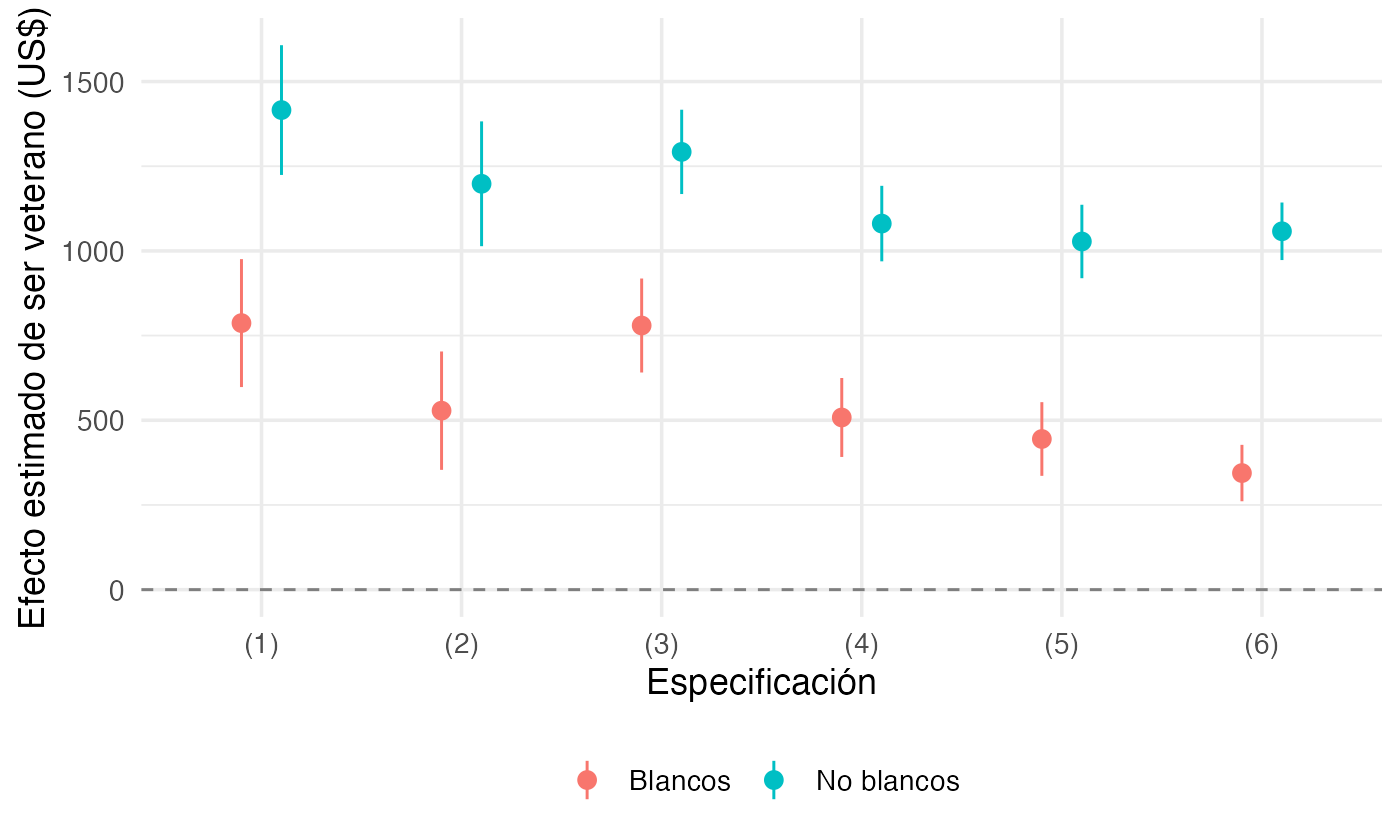
\includegraphics[width=0.68\textwidth]{figures/progression_plot.png}
		\end{center}
		\vspace{-0.2cm}
		\small Efecto estimado de $dvet$ con intervalo de confianza de 95\% en las seis especificaciones de la tabla.
	\end{frame}

	% --------------------------------------------------- Slide --
	\begin{frame}
		\frametitle{El signo del sesgo}
		\small
		\begin{itemize}
			\item Con una variable omitida $x_{2i}$ (el AFQT), el sesgo asint\'otico del coeficiente de la regresi\'on simple es
			\begin{align*}
				\text{Sesgo}(\hat \gamma_1)=\beta_2\frac{\Cov(dvet_{i},x_{2i})}{\Var(dvet_{i})}.
			\end{align*}
			\item <2-> Los coeficientes de los grupos AFQT son positivos y crecientes ($\beta_2>0$) y los veteranos tienen mayor puntaje ($\Cov(dvet_i,x_{2i})>0$).
			\item <3-> \alert{El sesgo es positivo}: la regresi\'on simple sobrestima el efecto del servicio militar.
			\item <3-> Con AFQT y escolaridad, el efecto estimado cae de $787$ a $508$ para blancos (35\%) y de $1,416$ a $1,081$ para no blancos (24\%).
		\end{itemize}
	\end{frame}

	% --------------------------------------------------- Slide --
	\begin{frame}
		\frametitle{Descomposici\'on del sesgo}
		\small
		\begin{itemize}
			\item Sea $\widehat \gamma_1$ el coeficiente de $dvet$ en la regresi\'on simple y $\widehat \beta_1$ en la regresi\'on con controles $z_{ji}$ (dummies de AFQT y escolaridad). En la muestra
			\begin{align*}
				\widehat \gamma_1 = \widehat \beta_1 + \sum_j \widehat \beta_j \, \widehat \delta_j,
			\end{align*}
			donde $\widehat \beta_j$ es el coeficiente de $z_{ji}$ en la regresi\'on con controles y $\widehat \delta_j$ es el coeficiente de $dvet_i$ en la regresi\'on de $z_{ji}$ sobre $dvet_i$.
			\item Cada t\'ermino $\widehat \beta_j \widehat \delta_j$ es lo que aporta la variable omitida $j$ al sesgo.
		\end{itemize}
		\begin{center}
			\scriptsize
			
\begin{tabular}{lccccc}
\toprule
Grupo & Regresi\'on simple & Con controles & Sesgo & Aporte AFQT & Aporte escolaridad\\
\midrule
Blancos & 786.9 & 508.3 & 278.6 & 256.5 & 22.2\\
No blancos & 1,415.8 & 1,080.7 & 335.1 & 206.1 & 129.0\\
\bottomrule
\end{tabular}

		\end{center}
		\vspace{-0.2cm}
		\small
		Para blancos casi todo el sesgo viene del AFQT. Para no blancos, tambi\'en aporta la escolaridad.
	\end{frame}

	% --------------------------------------------------- Slide --
	\begin{frame}
		\frametitle{M\'as controles, menos sesgo (pero no cero)}
		\small
		\begin{itemize}
			\item Las columnas (5) y (6) agregan cohorte, a\~no de solicitud y una dummy por cada celda de covariables: el efecto para blancos baja a $344$; para no blancos queda en torno a $1,050$.
			\item \term{Un solo sentido}: que el coeficiente se mueva al agregar controles es mala se\~nal para la regresi\'on simple. Que deje de moverse \emph{no prueba} que ya no haya sesgo: pueden quedar variables omitidas que no observamos (motivaci\'on, salud, alternativas laborales).
			\item El argumento de Angrist es que las fuerzas armadas seleccionan, sobre todo, con variables que s\'i observamos (edad, escolaridad, puntaje AFQT). \alert{Eso es una hip\'otesis sobre el proceso de selecci\'on, no algo que la regresi\'on verifique.}
		\end{itemize}
	\end{frame}

	% ============================================================
	\section{Efectos distintos por raza}
	% ============================================================

	% --------------------------------------------------- Slide --
	\begin{frame}
		\frametitle{Interacci\'on entre dummies}
		\small
		\begin{itemize}
			\item Un solo modelo con interacci\'on entre $dvet$ y $dnwhite$
			\begin{align*}
				\E(earnings|dvet,dnwhite)=\beta_0+\beta_{dvet}\,dvet+\beta_{dnwhite}\,dnwhite+\beta_{dvet\_dnwhite}\,dvet \times dnwhite.
			\end{align*}
			\item Estimaci\'on: $\hat\beta_{dvet}=787$, $\hat\beta_{dnwhite}=-2,272$ y $\hat\beta_{dvet\_dnwhite}=629$, con $\E(earnings)=12,431$.
			\item El efecto de $dvet$ es $\beta_{dvet}=787$ para blancos y $\beta_{dvet}+\beta_{dvet\_dnwhite}=1,416$ para no blancos: los mismos n\'umeros de la regresi\'on simple por raza.
			\item ?`Qu\'e mide $\beta_{dnwhite}$? ?`Y $\beta_{dvet\_dnwhite}$?
		\end{itemize}
	\end{frame}

	% ============================================================
	\section{Cierre}
	% ============================================================

	% --------------------------------------------------- Slide --
	\begin{frame}
		\frametitle{Resumen}
		\small
		\begin{itemize}
			\item La regresi\'on simple con una dummy es una diferencia de medias. Es causal solo si veteranos y no veteranos son comparables.
			\item Aqu\'i no lo son: \alert{selecci\'on positiva} (mayor AFQT) $\Rightarrow$ sesgo positivo de variable omitida.
			\item Agregar controles reduce el efecto estimado (35\% para blancos y 24\% para no blancos con AFQT y escolaridad), en la direcci\'on que predice el signo del sesgo.
			\item La descomposici\'on $\widehat \gamma_1 = \widehat \beta_1 + \sum_j \widehat \beta_j \widehat \delta_j$ dice cu\'anto aporta cada variable omitida.
			\item Angrist y Pischke (2009) reportan con las celdas ponderadas por su tama\~no: entre los blancos la diferencia de US\$1,233 se vuelve negativa al controlar por covariables, y entre los no blancos baja de US\$2,449 a US\$840. \alert{Las magnitudes cambian con la ponderaci\'on; el signo del sesgo y la lecci\'on no.}
		\end{itemize}
	\end{frame}

	% --------------------------------------------------- Slide --
	\begin{frame}
		\frametitle{Para discutir}
		\small
		\begin{itemize}
			\item ?`Por qu\'e el AFQT es la variable omitida m\'as importante para los blancos? ?`Qu\'e otras variables no observadas podr\'ian sesgar el resultado y en qu\'e direcci\'on?
			\item Si los solicitantes m\'as motivados son los que ingresan y tambi\'en los que m\'as ganan, ?`qu\'e signo tendr\'ia ese sesgo?
			\item ?`Qu\'e pasar\'ia con la regresi\'on simple si las fuerzas armadas aceptaran a los solicitantes por sorteo?
		\end{itemize}
	\end{frame}

	% --------------------------------------------------- Slide --
	\begin{frame}
		\frametitle{Datos y c\'odigo}
		\small
		\begin{itemize}
			\item Todo lo que aparece en estas diapositivas se genera con un script de R:
			\item [] \texttt{examples/4.MCO\_estimacion\_veteranos-angrist}
			\item \term{Fuente}:
			\begin{itemize}
				\item Angrist, J. (1998), ``Estimating the Labor Market Impact of Voluntary Military Service Using Social Security Data on Military Applicants'', \emph{Econometrica} 66(2): 249--288.
				\item Angrist, J. y J.-S. Pischke (2009), \emph{Mostly Harmless Econometrics}, cap. 3.3.1.
			\end{itemize}
		\end{itemize}
	\end{frame}

\end{document}
